% Revised Sections 3 and 4: preliminary complete-model comparisons.
% Figures use ordinary image files in the figures folder.
% Introduction and other unfinished sections retain the supplied prose.
\documentclass{article}


\usepackage{amsmath}
\usepackage{amsfonts}
\usepackage{amssymb}
\usepackage{graphicx}
\usepackage{subfigure}
\usepackage{booktabs}


%\usepackage{wsuipa}
\usepackage[usenames,dvipsnames]{xcolor}
\usepackage{fancybox}
\usepackage{tikz}
\usetikzlibrary{arrows,snakes,backgrounds}
\usepackage{hyperref}

\tikzstyle{place}=[circle,draw=blue!50,fill=blue!20,thick]
\pagestyle{plain} 
%%%%%%%%%% EXACT 1in MARGINS %%%%%%% 

\textheight235truemm\textwidth165truemm
\voffset-2.2cm\hoffset-1.2cm \vfuzz=10000truept\hfuzz=10000truept
\usepackage{lipsum}
\usepackage[usestackEOL]{stackengine}[2013-10-15]
\def\x{\hspace{1.5ex}}
\def\y{\hspace{1.225ex}}
\def\z{\hspace{1.9ex}}
\newcommand{\RED}[1]{{\color{red}{#1}}}
\newcommand{\ignore}[1]{}
\newcommand{\Matrix}[1]{\ensuremath{\left(\begin{array}{rrrrrrrrrrrrrrrrrr} #1 \end{array}\right)}}
\newcommand{\Matrixc}[1]{\ensuremath{\left(\begin{array}{cccccccccccc} #1 \end{array}\right)}}
\newcommand{\Matrixs}[1]{\ensuremath{\left[\begin{array}{cccccccccccc} #1 \end{array}\right]}}
\newcommand{\etal}{{\it et al.}}
\newcommand{\multiple}{{multiple} }

%\newcommand{\Kcomment}[1]{{\color{blue}{[KJ: #1]}}}

%\newcommand{\RED}[1]{{\color{red}{#1}}}
\def\proof{{\noindent \bf Proof.~}}
\def\endproof{\hspace{\fill}{\boldmath $\Box$}\par}

\newcommand{\GG}{{\mathcal{G}}}
\newcommand{\R}{{\mathbb{R}}}
\newcommand{\Z}{{\mathbb{Z}}}
\newtheorem{theorem}{Theorem}[section]
\newtheorem{lemma}[theorem]{Lemma}
\newtheorem{definition}[theorem]{Definition}
\newtheorem{corollary}[theorem]{Corollary}
\newtheorem{proposition}[theorem]{Proposition}
\newtheorem{remark}[theorem]{Remark}
\newtheorem{remarks}[theorem]{Remarks}
\newtheorem{example}[theorem]{Example}
\newtheorem{claim}[theorem]{Claim}



%\usepackage[
%backend=biber,
%style=alphabetic,
%sorting=ynt
%]{biblatex}
%\addbibresource{Chinese_med.bib}
%\addbibresource{network.bib}


\title{Is Lotka–Volterra-type of model right for five-element network in TMC?}
\author{Carter Feng and Yunjiao Wang}
%\date{}


\begin{document}

\maketitle
\begin{abstract}
    
\end{abstract}
\section{Introduction}

Traditional Chinese medicine (TCM) has been widely recognized  and becomes an invaluable component in alternative medicines in the west \cite{Kaptchuk2000} though it is not always viewed correctly.   Chinese medicine is the result of science over long time as it is the result of continuous critical thinking and extensive clinical observations and testing \cite{Kaptchuk2000}. It is a coherent and independent system of thoughts and practice that have been developed over 2000 years.   As Manfred Porkert \cite{Porkert1990} rightly pointed out, Chinese medicine is not less logical than the Western, just less analytical. 

TCM is an attractive alternative for several reasons.
First, TCM takes holistic approach, which takes into account of not only interactions among different components within the whole body, but also external environment such as season, time of the day, the place of living and so on. This approach is very different from that of modern medicine, which essentially treat a patient as an independent sick organ with a bunch of testing numbers. It is so often that disease spread from one organ to another. TCM has the principle that strengthen the still healthy organ that is directly impact by the ill organ before treat the sick one so to prevent spread. This can only be achieved by knowing the overall relations between the organs. Second, because of holistic approach, TCM natually uses multi-target approach instead of single-target as  modern medicine usually does (add citation). This approach could provide a balanced and effective treatment with less side effect. Third, TCM focuses on health, not disease. For example, it is so common that we feel something is going wrong, for example feeling lack of energy, but all medical tests show nothing wrong.  TCM focuses on identifying the root problems. As said in Huang Di Nei JIng, the best doctor is the one who bring patient back to true healthy before the patient even gets sick. 
Finally,  TCM  is very  accessible to average people. In the past, Chinese has some general idea on diagonizing and even able to construct some treatments by themselves for minor problems. 

Imagine that if everybody can identify themselves health issue before gets sick, then the immense cost in medical can be saved,  the pollution related to drugs can be dramatically reduced, and  people can live healthier and longer and happier.

TCM is developed based on theories and principles described in the ancient work Huang Di Nei Jing. The main theories are based on two networks: a five-node network called five-element system, and a two-node network called yin-yang relation.  Diagonsis and treatments are conducted based on the dynamics of the two networks.  In this work, we aims to introduce and understand the theories from network dynamics point of view. 

Network motif was proposed to understand dynamics of complex network systems by looking at small sub-networks that occur more often than usual or functionally building blocks \cite{milo2002, Alon2007}. It is  known that the dynamics of a sub-network  in general may not reflect the dynamics of the whole system. However, if the  sub-network is relatively independent, then its dynamics could be manifested in the dynamics of the whole system.  For example, the sub-network is an isolated network, or it does not have input from remaining networks. 
Interestingly, in TCM, major principles in diagnosis and treatments are based on the sub-networks  of the five-element network. 

The five-element network have been proposed to be modeled by a Boolean network system \cite{Bellavite1998}, or a system of differential equations \cite{Nian2025,Lin2020,zhang2011,Yang2025}.
We are interested in  Lotka–Volterra-type of model that was proposed in \cite{Lin2020}. Lin \etal \cite{Lin2020} studied the dynamics of the network at several special sets of parameters and explore possibility of chaotic dynamics. Their work was carried out from math interest instead of the applications in TMC.  To make a model meaningful, we need to make sure the model captures some key  characteristics  that are observed in applications. For example, a healthy system needs to be stable in the sense that perturb initial conditions, or perturb parameter values, the overall dynamics stay the same. 

In this work, we study equilibrium states and their stability of . 
explore the overall stability as we assume that a healthy human being should have stable dynamics. We thus explore overall stability of the system Lin's model and a modified version of the model. 

\section{The five-element network and principles in practice}

OUTLINE:

1. FIIVE - ELEMENT NETWORK

2. THE PRINCIPLES IN PRACTICE FOR TREATING ILLNESS

The five-element network consists of the five elements: wood, fire, earth, metal and water. 
\begin{figure}[!htb]
\centering
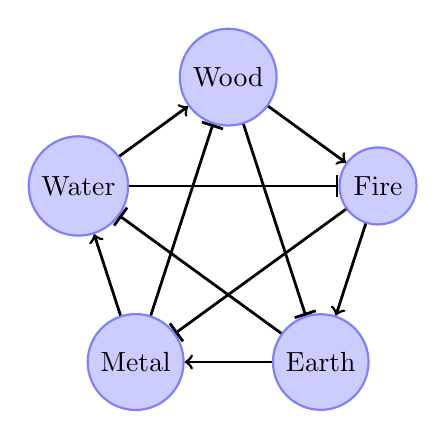
\begin{tikzpicture}[line width=1pt,  scale = 2]
\node[place] (M) at (90:1) {Wood};
\node[place]  (H) at (18:1) {Fire};
\node[place]  (J) at (234:1) {Metal};
\node[place]  (T) at (-54:1) {Earth};
\node[place]  (S) at ( 162:1) {Water};

\path[->] (M) edge (H)
        (H) edge (T)
            (T) edge  (J)
            (J) edge (S)
              (S) edge(M)
        (M) edge[-|] (T)
        (H) edge[-|] (J)
        (T) edge[-|]  (S)
        (J) edge[-|] (M)
        (S) edge[-|] (H);     
 \end{tikzpicture}

\caption{Five-element network  and motifs approach in practice}
\label{F:WuXing}
\end{figure}
The two types of arrows in the fig.~\ref{F:WuXing} represent two primary inter-element relationships: \textbf{Sheng (Generating $\to $) cycle.} and \textbf{Ke (Controlling, $\dashv$) cycle.}

{\bf Principles in practice.}
ADD THOSE DESCRIPTIONS

\section{Dynamics of Lin's Model}
\label{sec:lin-results}

The numerical results in this section and Section~\ref{sec:modified-results}
are preliminary comparisons of two complete five-node models under specified
parameter choices. They describe the existence and local stability of a
positive synchronous equilibrium and responses to selected initial
perturbations. Because the models differ in both interaction laws and the
presence of a direct child-loss term, these comparisons do not isolate the
mechanism responsible for a difference in stability. The coefficients used
below are illustrative and have not been calibrated to physiological data.

\subsection{Model, balanced equilibrium, and numerical protocol}
Let $x_i\geq0$ denote the activity of node $i$, with the nodes ordered as
Wood, Fire, Earth, Metal, and Water. All indices are taken modulo five.
In this ordering, $i-1$ is the generating predecessor (mother), $i+1$ is
the generating successor (child), $i-2$ is the controller, and $i+2$ is
the controlled target. The homogeneous six-term model of Lin and Han
\cite{Lin2020} is
\begin{equation}
\dot x_i=a x_i-bx_i^2+c x_i x_{i-1}-d x_i x_{i-2}
               -g x_i x_{i+1}-h x_i x_{i+2}.
\label{eq:lin-model}
\end{equation}
Both models studied here have five state variables; ``six-term'' refers to
the contributions to each equation, not to the number of nodes.
The nonnegative orthant is invariant for~\eqref{eq:lin-model} for as long
as the solution exists, since every component of its vector field contains
$x_i$ as a factor. This property does not imply boundedness or convergence.

We call $x=s\mathbf{1}$ a balanced, or synchronous, state. For $a>0$,
a positive balanced equilibrium exists precisely when
$M=b+d+g+h-c>0$, in which case
\begin{equation}
 s_{\mathrm L}=\frac{a}{b+d+g+h-c}.
 \label{eq:lin-balance}
\end{equation}
At this equilibrium the Jacobian is circulant. With
$\theta_j=2\pi j/5$, its eigenvalue real parts are
\begin{equation}
 \operatorname{Re}\lambda_j
 =s_{\mathrm L}\bigl[-b+(c-g)\cos\theta_j
                         -(d+h)\cos(2\theta_j)\bigr],
 \qquad j=0,\ldots,4.
 \label{eq:lin-spectrum}
\end{equation}
We use the spectral abscissa
$\alpha=\max_j\operatorname{Re}\lambda_j$ to assess local stability.
Strict negativity implies local exponential stability, whereas a positive
value implies instability. A zero real part requires further analysis.
The maps classify $\alpha<-10^{-9}$ as stable, $\alpha>10^{-9}$ as
unstable, and values between these thresholds as unresolved. Absence of a
positive synchronous equilibrium is recorded separately; it is not a
classification of the system's other equilibria or attractors.

For the trajectory comparisons, we used SciPy's DOP853 integrator with
relative tolerance $10^{-10}$ and absolute tolerance $10^{-12}$, and
sampled 3,001 times over $0\leq t\leq120$. A repeat with RK45 at the same
tolerances changed the sampled activities by at most $1.1\times10^{-8}$
across the four runs. Analytic Jacobians were checked by complex-step
differentiation at 1,000 random states per model; the largest absolute
entrywise discrepancy was below $8\times10^{-15}$. These checks support
the implementation, but do not establish global dynamical conclusions.

\subsection{Baseline stability and response to initial perturbations}
At the illustrative Lin baseline
$(a,b,c,d,g,h)=(1,1,1,1,1,1)$, the positive balanced level is
$s_{\mathrm L}=1/3$. The leading pair is approximately
$0.206011\pm0.634038\,\mathrm{i}$, so this equilibrium is unstable
(Figure~\ref{fig:baseline-spectra}).
For comparison, the modified-model spectrum shown in the same figure uses
the separate baseline specified in Section~\ref{sec:modified-stability}.

\begin{figure}[tbp]
\centering
\includegraphics[width=\linewidth]{figures/figure1.png}
\caption{Jacobian eigenvalues at the stated positive balanced equilibria.
Lin: $(a,b,c,d,g,h)=(1,1,1,1,1,1)$ and $s_{\mathrm L}=1/3$.
Modified: $(a,k,c,g,h)=(2,0.5,1,0.5,0.3)$ and
$s_{\mathrm D}=(3+\sqrt{59})/4$.
The vertical line is $\operatorname{Re}\lambda=0$.
These are local stability results at different illustrative baselines,
not a matched-parameter test of a single interaction mechanism.}
\label{fig:baseline-spectra}
\end{figure}

We then initialized each model at its own balanced equilibrium and changed
only Wood: either $x_1(0)=1.05s$ or $x_1(0)=0.30s$, keeping
$x_i(0)=s$ for $i=2,\ldots,5$.
In the Lin runs, the solutions moved away from balance and exhibited
sustained oscillatory behavior over the observation interval
(Figure~\ref{fig:disturbance}). The distances
$\lVert x(120)-s_{\mathrm L}\mathbf{1}\rVert_2$ were approximately
$0.8776$ and $0.9899$, respectively. These trajectories illustrate the
baseline equilibrium's instability. They do not imply that the model lacks
stable equilibria at other parameters, or that an unstable equilibrium
necessarily produces unbounded activity or chaos.

\begin{figure}[tbp]
\centering
\includegraphics[width=\linewidth]{figures/figure2.png}
\caption{Responses to a one-component initial disturbance, using the
baselines in Figure~\ref{fig:baseline-spectra}. Top: Wood increased by
$5\%$; bottom: Wood reduced to $30\%$ of its balanced value. Other
components start at balance. Activities are divided by the relevant
balanced level $s$. All runs extend to $t=120$; the modified-model panels
show only $0\leq t\leq12$ to make recovery visible. Each curve represents
one of the five nodes. These are specified finite perturbations, not a
basin-wide or globally uniform recovery test.}
\label{fig:disturbance}
\end{figure}

\subsection{Stability under a two-parameter sweep}
To explore parameter dependence, we varied nourishment $c$ and received
restraint $d$ on a $90\times90$ equally spaced grid,
\begin{equation}
 c\in[0.3,1.6],\qquad d\in[0.1,1.0],\qquad
 a=1.5,\quad b=0.65,\quad g=h=0.3.
 \label{eq:lin-sweep}
\end{equation}
The Lin panel of Figure~\ref{fig:stability-maps} shows the resulting
stability landscape. Of 8,100 grid points, 7,867 admitted a positive balanced
equilibrium and 1,497 were locally stable. Thus stable positive balance
occurred at $18.5\%$ of all sampled points, or $19.0\%$ of those admitting
positive balance. The remaining 233 points lacked a positive synchronous
equilibrium. These percentages describe this finite grid, not an intrinsic
probability of stability for Lin's model.

Stable positive balance is therefore possible in Lin's model. For example,
$(a,b,c,d,g,h)=(1,2,1,1,1,1)$ gives $s_{\mathrm L}=0.25$ and
$\alpha\approx-0.095492$. Conclusions drawn from the all-ones baseline
must not be extended to all parameter choices.

\subsection{Status of motif analysis}
The present results concern the full five-node system. A completed stability
comparison of two-node motifs is not included here. Such a comparison must
first specify whether the remaining nodes are deleted or clamped to fixed
background activities, since these operations define different reduced
systems. Motif dynamics are left for subsequent analysis.

\section{A modified version of the model and its dynamics}
\label{sec:modified-results}

\subsection{Five-term model and nonnegative activities}
The modified model considered in all results below is
\begin{equation}
 \dot x_i=a x_i-kx_i^2+\frac{c x_{i-1}}{1+x_i}
                  -\frac{g x_i}{1+x_{i+2}}-h x_i x_{i-2},
 \qquad i=1,\ldots,5.
 \label{eq:modified-model}
\end{equation}
We assume positive coefficients and nonnegative initial activities.
The generating input is linear in predecessor activity and decreases with
recipient activity. The target-dependent loss is moderated by target
activity, while received restraint remains bilinear.
At $x_i=0$, the right-hand side is $c x_{i-1}\geq0$, so the nonnegative
orthant is invariant. Moreover, at a component attaining the maximum
$X=\max_i x_i$, its derivative is bounded above by
$aX-kX^2+c$. Consequently, for $k>0$, nonnegative solutions remain bounded
by $\max\{\max_i x_i(0),B\}$, where
\begin{equation}
 B=\frac{a+\sqrt{a^2+4kc}}{2k}.
\end{equation}
This establishes a nonnegative, bounded activity domain; it does not imply
global convergence to a particular equilibrium.

Equation~\eqref{eq:modified-model} makes several simultaneous changes to
Lin's model. It omits the direct child-loss term and changes both the
predecessor input and the target-dependent loss. In particular, the
partial derivative with respect to target activity is positive in the
modified model, whereas it is negative in Lin's model. Also, the symbols
$g$ and $h$ do not denote the same terms in the two equations:
received restraint has coefficient $d$ in Lin and $h$ in the modified
model. These differences must be considered when interpreting the plots.

\subsection{Balanced equilibrium and baseline stability}
\label{sec:modified-stability}
The origin is an equilibrium. For a nonzero synchronous equilibrium
$x=s\mathbf{1}$, the balanced level satisfies
\begin{equation}
 (k+h)s^2+(k+h-a)s-(a+c-g)=0.
 \label{eq:modified-balance}
\end{equation}
The maps use the larger positive root, when it exists. There is a unique
positive root when $a+c>g$; other parameter choices can admit two positive
roots, so this condition is sufficient but not necessary for positive
balance. At a balanced level $s$, set
\[
 D_0=a-2ks-\frac{cs}{(1+s)^2}-\frac{g}{1+s}-hs.
\]
The eigenvalue real parts are
\begin{equation}
 \operatorname{Re}\lambda_j
 =D_0+\frac{c}{1+s}\cos\theta_j
       +s\left(\frac{g}{(1+s)^2}-h\right)\cos(2\theta_j).
 \label{eq:modified-spectrum}
\end{equation}
At $(a,k,c,g,h)=(2,0.5,1,0.5,0.3)$,
$s_{\mathrm D}=(3+\sqrt{59})/4\approx2.670286$ and
$\alpha\approx-1.153724$. All five eigenvalues have negative real parts
(Figure~\ref{fig:baseline-spectra}), establishing local exponential
stability at this baseline.

For the same relative Wood perturbations used in
Section~\ref{sec:lin-results}, both modified-model trajectories returned
to this equilibrium. Their final distances at $t=120$ were approximately
$3.3\times10^{-12}$ and $1.2\times10^{-11}$
(Figure~\ref{fig:disturbance}). This supports recovery from the two tested
initial conditions. Since the baselines have different coefficient values
and equilibrium scales, the displayed decay and oscillation rates do not
provide a calibrated comparison of physiological recovery times.

\subsection{Stability maps and sensitivity to parameter sampling}
For the modified-model panel of Figure~\ref{fig:stability-maps}, we used
\begin{equation}
 c\in[0.3,1.6],\qquad h\in[0.1,1.0],\qquad
 a=1.5,\quad k=0.65,\quad g=0.3,
 \label{eq:modified-sweep}
\end{equation}
on the same $90\times90$ grid. Every sampled point admitted a positive
balanced equilibrium and was locally stable. Thus, in these specified
slices, the modified model had a larger sampled region of stable positive
balance than Lin's model. This does not establish stability for all
parameters. For example, the earlier modified-model sweep with
$a=2$, $k=0.5$, $g=0.5$, $c\in[0.05,2.5]$, and $h\in[0.05,2.0]$
had 5,837 stable points out of 8,100 ($72.1\%$); all those points admitted
positive balance. The different percentages reflect different experiments.

\begin{figure}[tbp]
\centering
\includegraphics[width=\linewidth]{figures/figure3.png}
\caption{Stability maps on the verified $90\times90$ parameter grids.
Horizontal axis: nourishment $c$. Vertical axis: received restraint,
meaning $d$ in Lin and $h$ in the modified model.
Lin uses $(a,b,c,d,g,h)=(1.5,0.65,c,d,0.3,0.3)$; the modified model uses
$(a,k,c,g,h)=(1.5,0.65,c,0.3,h)$. Colors show the largest real part of
the Jacobian eigenvalues at the selected positive balanced equilibrium:
blue indicates negative values and red positive values. Color limits are
clipped, so the darkest colors also represent values beyond the displayed
scale. Gray denotes no positive balanced equilibrium; the black line is
an interpolated zero contour. Titles give the stable fraction among all
grid points, while inset labels condition on existence of positive balance.
These are specified slices of different complete models, including a fixed
child-loss coefficient $g=0.3$ in Lin; they do not isolate a single change
in interaction law.}
\label{fig:stability-maps}
\end{figure}

We also summarized sensitivity to three illustrative parameter distributions
(Figure~\ref{fig:sampling} and Table~\ref{tab:sampling}). For a shared conceptual draw
$(S,A,C,R,T,L)$, representing self-growth, self-limitation, nourishment,
received restraint, target-related loss, and child loss, the parameter
assignments were
\[
 (a,b,c,d,g,h)_{\mathrm L}=(S,A,C,R,L,T),\qquad
 (a,k,c,g,h)_{\mathrm D}=(S,A,C,T,R).
\]
The uniform scenario draws all six quantities independently from
$[0.1,2]$. The ordered scenario uses the same draws conditioned on
$S>C>R>T$, without ordering $A$ or $L$. The tiered scenario draws
independently from $S\in[1,2]$, $A\in[0.3,1]$, $C\in[0.5,1.5]$,
$R\in[0.2,0.8]$, and $T,L\in[0.1,0.5]$.
Each scenario uses 1,200 accepted draws and NumPy's default random-number
generator with seed 3. The two models share each conceptual draw, but
there is no child-loss coefficient in the modified model. This pairing
specifies the experiment; it does not equate the strengths of different
functional forms or remove the structural difference.

\begin{table}[tbp]
\centering
\small
\begin{tabular}{llrrr}
\toprule
Scenario & Model & Stable / eligible & Stable / eligible (\%) & Stable / all (\%)\\
\midrule
Uniform & Lin      & 273 / 1195  & 22.8 & 22.8\\
        & Modified & 968 / 1029  & 94.1 & 80.7\\
Ordered & Lin      & 562 / 1192  & 47.1 & 46.8\\
        & Modified & 1103 / 1200 & 91.9 & 91.9\\
Tiered  & Lin      & 267 / 1145  & 23.3 & 22.2\\
        & Modified & 1188 / 1200 & 99.0 & 99.0\\
\bottomrule
\end{tabular}
\caption{Stability frequencies under the stated sampling assumptions.
``Eligible'' means that the selected positive synchronous equilibrium
exists; ``all'' means all 1,200 draws in that scenario. The counts retain
both denominators, so failure to admit positive balance is not silently
excluded. These are parameter-sampling results, not physiological
probabilities or evidence of universal superiority.}
\label{tab:sampling}
\end{table}


\begin{figure}[tbp]
\centering
\includegraphics[width=\linewidth]{figures/figure4.png}
\caption{Stability frequencies under the uniform, ordered, and tiered
sampling schemes described in the text, with 1,200 draws per scheme and
seed 3. Left: the fraction with a locally stable positive balanced
equilibrium among draws admitting the selected positive balance. Right:
the fraction among all 1,200 draws. Exact counts are given in
Table~\ref{tab:sampling}. These percentages depend on the sampling
assumptions and eligibility rule; they are not probabilities that a model
is correct or physiologically healthy. The comparison changes several
mechanisms simultaneously and does not attribute the differences to one
interaction law.}
\label{fig:sampling}
\end{figure}

\subsection{Interpretation and limitations of the preliminary comparison}
The results establish a limited numerical observation: for the specified
baselines, parameter slices, and sampling distributions, the modified
model more often admits a locally stable positive balanced equilibrium,
and it recovers from the two tested disturbances at its selected baseline.
They do not show that demand modulation alone produces these differences.
The comparison simultaneously changes interaction laws, removes the
child-loss term, and, in the baseline examples, changes parameter values.
Equal numerical coefficients multiplying different functions do not by
themselves constitute a calibration. The size of a stable region also
depends on the chosen coordinates, parameter window, and sampling measure.

A mechanism-focused comparison would first use a matched bilinear model
with the same five terms as~\eqref{eq:modified-model}, and then vary the
interaction laws separately. Removing the child-loss term from Lin's
model gives this comparator after relabeling coefficients. Such a study
would distinguish the effect of that removal from the effects of changing
the input and target-dependent loss laws. It is not the experiment shown
by the current Lin comparison diagrams. We therefore present these
figures as preliminary descriptions of two complete models, without
attributing their differences to a single cause or interpreting local
stability as clinical validation. As in Section~\ref{sec:lin-results},
the corresponding motif analysis remains to be completed.


\section{Conclusion and Discussion}

\section{Acknowledgments}
%\printbibliography

%\bibliographystyle{spbasic}      % basic style, author-year citations
\bibliographystyle{plain}      % mathematics and physical sciences
%\bibliographystyle{spphys}       % APS-like style for physics
% The original bibliography files were not supplied with the pasted source.
% Restore both .bib files for the complete introduction bibliography.
\IfFileExists{Chinese_med.bib}{%
  \IfFileExists{network.bib}{\bibliography{Chinese_med,network}}{\begin{thebibliography}{99}
\bibitem{Lin2020} H. Lin and J. Han.
Analysis of Dynamic Five-Element Model.
In \emph{Proceedings of the 39th Chinese Control Conference},
pages 777--781, 2020.
\href{https://doi.org/10.23919/CCC50068.2020.9188438}{doi:10.23919/CCC50068.2020.9188438}.
\end{thebibliography}}%
}{\begin{thebibliography}{99}
\bibitem{Lin2020} H. Lin and J. Han.
Analysis of Dynamic Five-Element Model.
In \emph{Proceedings of the 39th Chinese Control Conference},
pages 777--781, 2020.
\href{https://doi.org/10.23919/CCC50068.2020.9188438}{doi:10.23919/CCC50068.2020.9188438}.
\end{thebibliography}}



\end{document} 